\documentclass{beamer}

\usetheme{Madrid} % Singapore, Madrid, Ilmenau, CambridgeUS
\setbeamertemplate{navigation symbols}{}

% --- Colores personalizados ---
\definecolor{unahurverde}{HTML}{005C5C}
\definecolor{unahurgris}{HTML}{EAEAEA}
\setbeamercolor{structure}{fg=unahurverde}
\setbeamercolor{frametitle}{bg=unahurverde, fg=white}
\setbeamercolor{title}{fg=unahurverde}
\setbeamercolor{block title}{bg=unahurverde, fg=white}
\setbeamercolor{block body}{bg=unahurgris, fg=black}

% --- Logo en esquina superior derecha ---
\addtobeamertemplate{frametitle}{}{%
	\begin{textblock*}{3cm}(11.88cm,0.12cm)
		
\includegraphics[height=0.7cm]{logo_unahur.png}
	\end{textblock*}
}

\setbeamertemplate{caption}[numbered]


\usepackage[utf8]{inputenc}
\usepackage[spanish]{babel}
\usepackage{graphicx}
\usepackage{ragged2e}
\usepackage[table]{xcolor}
\usepackage{listings}
\usepackage{caption}
\usepackage{enumitem}
\usepackage[absolute,overlay]{textpos} % Necesario para el logo

\usefonttheme[onlymath]{serif}

\definecolor{codegray}{rgb}{0.5,0.5,0.5}
\definecolor{backcolor}{rgb}{0.95,0.95,0.95}
\definecolor{verdecelda}{HTML}{B7CBA6}
\definecolor{rojocelda}{HTML}{FF9999}
\definecolor{lightgray}{gray}{0.6}

\definecolor{codebg}{rgb}{0.95,0.97,0.98}       % fondo celeste muy suave
\definecolor{codecomment}{rgb}{0.42,0.55,0.34}  % verde oliva suave y cursiva
\definecolor{codekeyword}{rgb}{0.0,0.45,0.73}    % azul turquesa
\definecolor{codestring}{rgb}{0.78,0.36,0.14}   % naranja marrón claro
\definecolor{codenumber}{rgb}{0.5,0.5,0.5}      % gris numeración
\definecolor{coderule}{rgb}{0.7,0.8,0.9}        % borde celeste suave

\lstdefinestyle{mystyle}{
	backgroundcolor=\color{codebg},
	commentstyle=\color{codecomment},
	keywordstyle=\color{codekeyword}\bfseries,
	stringstyle=\color{codestring},
	numberstyle=\tiny\color{codenumber},
	basicstyle=\ttfamily\footnotesize,
	breaklines=true,
	captionpos=b,
	keepspaces=true,
	numbersep=7pt,
	showspaces=false,
	showstringspaces=false,
	showtabs=false,
	tabsize=2,
	inputencoding=utf8,
	extendedchars=true,
	frame=single,
	rulecolor=\color{coderule},
	numbers=none,
	xleftmargin=10pt,
	literate={π}{{$\pi$}}1 {θ}{{$\theta$}}1 {μ}{{$\mu$}}1 {β}{{$\beta$}}1 {η}{{$\eta$}}1 {δ}{{$\delta$}}1 {Δ}{{$\Delta$}}1
	{á}{{\'a}}1 {é}{{\'e}}1 {í}{{\'i}}1 {ó}{{\'o}}1 {ú}{{\'u}}1
	{Á}{{\'A}}1 {É}{{\'E}}1 {Í}{{\'I}}1 {Ó}{{\'O}}1 {Ú}{{\'U}}1
	{ñ}{{\~n}}1 {Ñ}{{\~N}}1 {ζ}{{$\zeta$}}1
}

\lstset{style=mystyle}

\lstset{
	language=Python,
	emph={self, _aplicar_gamma, _escalar_255, _generar_vector_ruido}, emphstyle=\color{purple}\bfseries,
}

\title{Trabajo Práctico 1 Procesamiento de Imágenes y Visión por Computadora}
\author{Matías Cisnero}
\date{11 de agosto de 2025}

\begin{document}
	
	% Portada
\begin{frame}
	\centering
	
\includegraphics[width=0.25\textwidth]{UNAHUR.png}
	\vfill
	{\huge \textbf{Trabajo Práctico 1}}\\[0.2cm]
	{\Large Procesamiento de Imágenes y Visión por Computadora}\\
	\vfill
	{\large Matías Cisnero}\\
	{\small 11 de agosto de 2025}
\end{frame}
	
\section{Ejercicio 1}
	
\begin{frame}
	\begin{center}
		\textcolor{unahurverde}{\textbf{Consigna 1:}}
	\end{center}
	\justifying
	
	Implementar la función de potencia $\gamma, 0 < \gamma < 2$ y $\gamma \neq 1$.
\end{frame}

\begin{frame}[fragile]{Transformación Gamma $\gamma$}
	\justifying

	\begin{block}{Definición}
		\[
		T(r) = c \, r^\gamma, \quad 0 < \gamma < 2, \ \gamma \neq 1
		\]
	\end{block}
	
	Donde $c$ es una constante apropiada, de tal forma que $T(255) = 255$.
	
	\begin{block}{Constante $c$}
		\[
		c = 255^{1-\gamma}
		\]
	\end{block}
	
	Y $r$ los niveles de gris de una imagen $f$.
\end{frame}

\begin{frame}[fragile]{Código}
	\justifying
	
	\begin{lstlisting}[language=Python]
def _aplicar_gamma(self, imagen, gamma):
	# Convierto en un array de (m, n, 3)
	imagen_np = np.array(imagen)
			
	c = (255)**(1-gamma)
	resultado_np = c*(imagen_np**gamma)
			
	self.imagen_procesada = Image.fromarray(resultado_np.astype('uint8'))
	\end{lstlisting}
	
 \vfill
	\footnotesize \textcolor{lightgray}{(*) Se puede operar directamente con la imagen gracias al Broadcasting de Numpy (ver \cite{numpy-broadcasting}).}
\end{frame}

\begin{frame}[fragile]{Resultados}
	\justifying
	Al aplicar la transformación con $\gamma = 1.5$ en la Figura~\ref{fig:lenaoriginal1} obtenemos la imagen de la Figura~\ref{fig:lenaej1}:
	\vspace{0.5cm}
	
	\centering
	\begin{minipage}{0.45\linewidth}
		\centering
		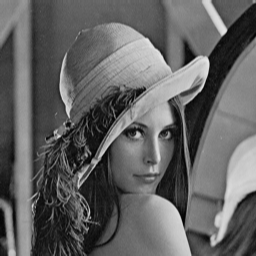
\includegraphics[width=\linewidth]{../results/lena_original}
		\captionof{figure}{Imagen original}
		\label{fig:lenaoriginal1}
	\end{minipage}\hfill
	\begin{minipage}{0.45\linewidth}
		\centering
		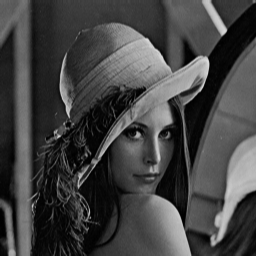
\includegraphics[width=\linewidth]{../results/lena_ej1}
		\captionof{figure}{Imagen modificada}
		\label{fig:lenaej1}
	\end{minipage}
\end{frame}

\section{Ejercicio 2}

\begin{frame}
	\begin{center}
		\textcolor{unahurverde}{\textbf{Consigna 2:}}
	\end{center}
	\justifying
	
	Implementar una función que devuelva el negativo de una imagen.
\end{frame}

\begin{frame}[fragile]{Negativo}
	\justifying
	
	\begin{block}{Definición}
		\[
		T(r) = 255 - r
		\]
	\end{block}
\end{frame}

\begin{frame}[fragile]{Código}
	\justifying
	
	\begin{lstlisting}[language=Python]
def _aplicar_negativo(self):
	# Convierto en un array de (m, n, 3)
	imagen_np = np.array(self.imagen_procesada)
	
	resultado_np = 255 - imagen_np
	self.imagen_procesada = Image.fromarray(resultado_np.astype('uint8'))
	\end{lstlisting}
	
	\vfill
	\footnotesize \textcolor{lightgray}{(*) Nuevamente se puede operar directamente gracias al Broadcasting de Numpy (ver \cite{numpy-broadcasting}).}
\end{frame}

\begin{frame}[fragile]{Resultados}
	\justifying
	Al aplicar el negativo en la Figura~\ref{fig:lenaoriginal2} obtenemos la imagen de la Figura~\ref{fig:lenaej2}:
	\vspace{0.5cm}
	
	\centering
	\begin{minipage}{0.45\linewidth}
		\centering
		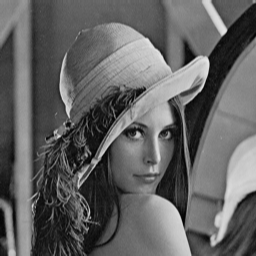
\includegraphics[width=\linewidth]{../results/lena_original}
		\captionof{figure}{Imagen original}
		\label{fig:lenaoriginal2}
	\end{minipage}\hfill
	\begin{minipage}{0.45\linewidth}
		\centering
		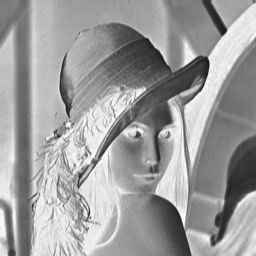
\includegraphics[width=\linewidth]{../results/lena_ej2}
		\captionof{figure}{Imagen en negativo}
		\label{fig:lenaej2}
	\end{minipage}
\end{frame}

\section{Ejercicio 3}

\begin{frame}
	\begin{center}
		\textcolor{unahurverde}{\textbf{Consigna 3:}}
	\end{center}
	\justifying
	
	Implementar una función que devuelva el histograma de niveles de gris de una imagen.
\end{frame}

\section{Ejercicio 4}

\begin{frame}
	\begin{center}
		\textcolor{unahurverde}{\textbf{Consigna 4:}}
	\end{center}
	\justifying
	
	Implementar una función que aplique un umbral a una imagen, devolviendo una imagen binaria. El umbral debe ser un parámetro de entrada.
\end{frame}

\begin{frame}[fragile]{Umbralización}
	\justifying
	
	\begin{block}{Definición}
		Dado un umbral $u \in [0,...,255]$
		\[
		T(r) =
		\begin{cases}
			255, & \text{si } r \geq u \\
			0, & \text{si } r < u
		\end{cases}
		\]
	\end{block}
\end{frame}

\begin{frame}[fragile]{Código}
	\justifying
	
	\begin{lstlisting}[language=Python]
def _aplicar_umbralizacion(self, imagen, umbral):
	# Convierto en un array de (m, n, 3)
	imagen_np = np.array(imagen)
	
	resultado_np = np.where(imagen_np >= umbral, 255, 0)
	
	self.imagen_procesada = Image.fromarray(resultado_np.astype('uint8'))
	\end{lstlisting}
	
	\vfill
	\footnotesize \textcolor{lightgray}{(*) np.where es una forma vectorizada de hacer un if-else para los píxeles de la imagen (ver \cite{numpy-where}).}\\
	\footnotesize \textcolor{lightgray}{(*) El umbral se asigna mediante un Scale (slider) de tkinter.}
\end{frame}

\begin{frame}[fragile]{Resultados}
	\justifying
	Al aplicar la umbralización con $u=128$ en la Figura~\ref{fig:lenaoriginal4} obtenemos la imagen de la Figura~\ref{fig:lenaej4}:
	\vspace{0.5cm}
	
	\centering
	\begin{minipage}{0.45\linewidth}
		\centering
		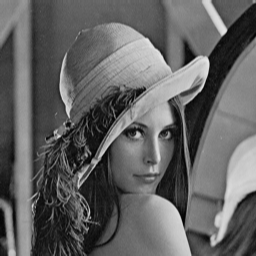
\includegraphics[width=\linewidth]{../results/lena_original}
		\captionof{figure}{Imagen original}
		\label{fig:lenaoriginal4}
	\end{minipage}\hfill
	\begin{minipage}{0.45\linewidth}
		\centering
		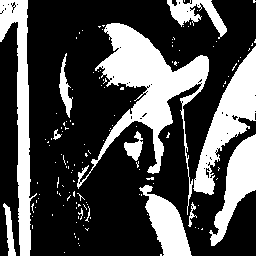
\includegraphics[width=\linewidth]{../results/lena_ej4}
		\captionof{figure}{Imagen en negativo}
		\label{fig:lenaej4}
	\end{minipage}
\end{frame}

\section{Ejercicio 5}

\begin{frame}
	\begin{center}
		\textcolor{unahurverde}{\textbf{Consigna 5:}}
	\end{center}
	\justifying
	
	Implementar una función que realice la ecualización del histograma para mejorar la imagen.
\end{frame}

\begin{frame}[fragile]{Ecualización del histograma}
	\justifying
	
	\begin{block}{Definición}
		\[
		s_k = T(r_k) = \sum_{i=0}^{k} \frac{n_i}{n}
		\]
	\end{block}
	
	donde:
	
	\begin{itemize}
		\item $r_k$ es el k-ésimo nivel de gris dentro del intervalo [0, 255].
		\item $n_i$, $i=0,...,255$ es el número de pixels de la imagen con nivel de gris $r_i$, $i=0,...,255$.
		\item $n$ es el número total de pixels de la imagen.
		\item $\frac{n_i}{n}$, $i=0,...,255$ es la frecuencia relativa del i-ésimo nivel de gris.
	\end{itemize}
	
	Actualmente $s_{min} \leq s_k \leq 1$ y queremos que $s_k \in [0, 255]$, para eso aplicamos la siguiente transformación para discretizar los valores:
	
	\[
	\hat{s_k} = 255 * \lceil \frac{s_k - s_{min}}{1 - s_{min}} \rceil
	\]
\end{frame}

\begin{frame}[fragile]{Código}
	\justifying
	
	\begin{lstlisting}[language=Python]
def _aplicar_ecualizacion_histograma(self):
	imagen_np_gris = np.array(self.imagen_procesada.convert('L')) # Array de la forma (m. n).
	datos_gris = imagen_np_gris.flatten()
	
	n_r = np.bincount(datos_gris, minlength=256) # Freq abs(ni)
	NM = datos_gris.size # Pixels totales(n)
	h_r = n_r / NM # Freq relativa(ni/n)
	
	sk = np.zeros(256) # Hacemos la suma acumulada
	for k in range(len(sk)):
		sk[k] = np.sum(h_r[0:k+1])
	
	sk_sombrero = self._escalar_255(sk) # Discretizamos
	resultado_np = sk_sombrero[imagen_np_gris]
	
	self.imagen_procesada = Image.fromarray(resultado_np.astype('uint8')).convert('RGB')
	\end{lstlisting}
\end{frame}

\begin{frame}[fragile]{Código +}
	\justifying
	Una forma más optimizada de hacerlo aprovechando los métodos de Numpy.
	
	\begin{lstlisting}[language=Python]
def _aplicar_ecualizacion_histograma(self):
	imagen_np_gris = np.array(self.imagen_procesada.convert('L'))
	datos_gris = imagen_np_gris.flatten()
	
	n_r = np.bincount(datos_gris, minlength=256) # Freq abs
	h_r = n_r / np.sum(n_r) # Freq relativa
	
	sk = np.cumsum(h_r)
	sk_sombrero = self._escalar_255(sk) # Discretizamos
	
	resultado_np = sk_sombrero[imagen_np_gris]
	self.imagen_procesada = Image.fromarray(resultado_np.astype('uint8')).convert('RGB')
	\end{lstlisting}
	
	\vfill
	\footnotesize \textcolor{lightgray}{(*) np.cumsum hace la suma acumulada desde el principio hasta la posición del valor (ver \cite{numpy-cumsum}). np.bincount cuenta la cantidad de veces que aparece cada valor con indice igual a nivel de pixel y valor igual a frecuencia (ver \cite{numpy-bincount}).}
\end{frame}

\begin{frame}[fragile]{Resultados histogramas}
	\justifying
	Al realizar la ecualización del histograma de la Figura~\ref{fig:hist_original} obtenemos el de la Figura~\ref{fig:hist_ecualizado}:
	\vspace{0.5cm}
	
	\centering
	\begin{minipage}{0.45\linewidth}
		\centering
		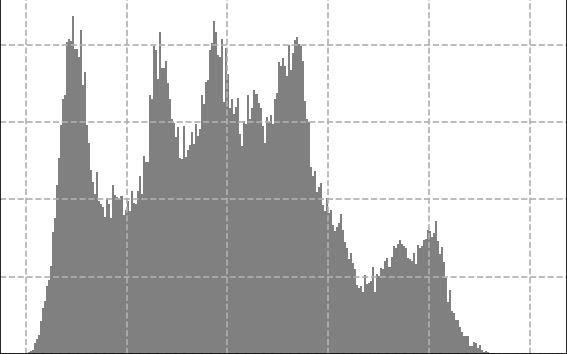
\includegraphics[width=\linewidth]{../results/lena_hist_gris}
		\captionof{figure}{Histograma original}
		\label{fig:hist_original}
	\end{minipage}\hfill
	\begin{minipage}{0.45\linewidth}
		\centering
		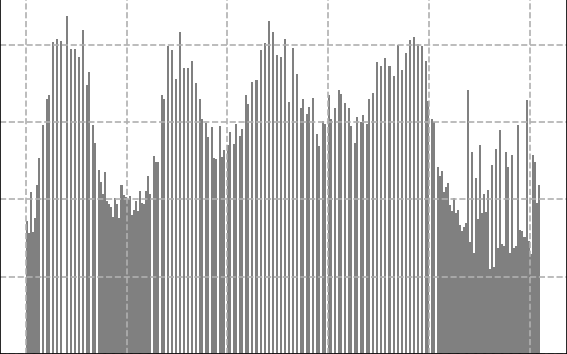
\includegraphics[width=\linewidth]{../results/lena_hist_gris_ecualizado}
		\captionof{figure}{Histograma ecualizado}
		\label{fig:hist_ecualizado}
	\end{minipage}
\end{frame}

\begin{frame}[fragile]{Resultados imagen}
	\justifying
	La ecualización de la imagen se puede apreciar al ver como al ecualizar la Figura~\ref{fig:lenaoriginal5} se obtiene la Figura~\ref{fig:lenaej5}:
	\vspace{0.5cm}
	
	\centering
	\begin{minipage}{0.45\linewidth}
		\centering
		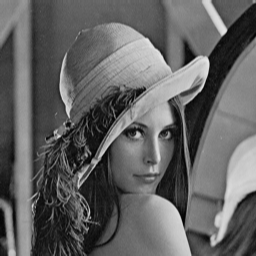
\includegraphics[width=\linewidth]{../results/lena_original}
		\captionof{figure}{Imagen original}
		\label{fig:lenaoriginal5}
	\end{minipage}\hfill
	\begin{minipage}{0.45\linewidth}
		\centering
		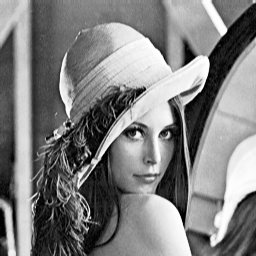
\includegraphics[width=\linewidth]{../results/lena_ej5}
		\captionof{figure}{Imagen ecualizada}
		\label{fig:lenaej5}
	\end{minipage}
\end{frame}

\section{Ejercicio 6}

\begin{frame}
	\begin{center}
		\textcolor{unahurverde}{\textbf{Consigna 6:}}
	\end{center}
	\justifying
	
	Aplicar la ecualización del histograma por segunda vez a la misma imagen.  
	Observar el resultado y dar una explicación de lo sucedido.
\end{frame}

\section{Ejercicio 7}

\begin{frame}
	\begin{center}
		\textcolor{unahurverde}{\textbf{Consigna 7:}}
	\end{center}
	\justifying
	
	Implementar generadores de números aleatorios con las siguientes distribuciones:
	
	\begin{enumerate}[label=\alph*)]
		\item Gaussiana con desviación estándar $\sigma$ y valor medio $\mu$.
		\item Rayleigh con parámetro $\xi$.
		\item Exponencial con parámetro $\lambda$.
	\end{enumerate}
	
	\vspace{0.3cm}
	
	Luego graficar los histogramas correspondientes.  
	Puede utilizarse una librería que genere números aleatorios.  
	Los parámetros del generador deben ser parámetros de entrada.
\end{frame}

\begin{frame}[fragile]{Código}
	\justifying
	Para generar los números aleatorios (1000) con las distribuciones correspondientes se realizó la siguiente función:
	
	\begin{lstlisting}[language=Python]
def _generar_vector_ruido(self, distribucion, intensidad, cantidad):
	# distribucion = np.random.normal, np.random.rayleigh, np.random.exponential
	vector_aleatorio = distribucion(scale=intensidad, size=(cantidad, 1))
	
	return vector_aleatorio
	\end{lstlisting}
	
	\vfill
	\footnotesize \textcolor{lightgray}{(*) en np.random.normal el parámetro "loc" predeterminadamente es 0.}
\end{frame}

\begin{frame}[fragile]{Resultados}
	\justifying
	Los histogramas obtenidos fueron:
	\vspace{0.3cm}
	
	\centering
	% Primera imagen
	\begin{minipage}{0.32\linewidth}
		\centering
		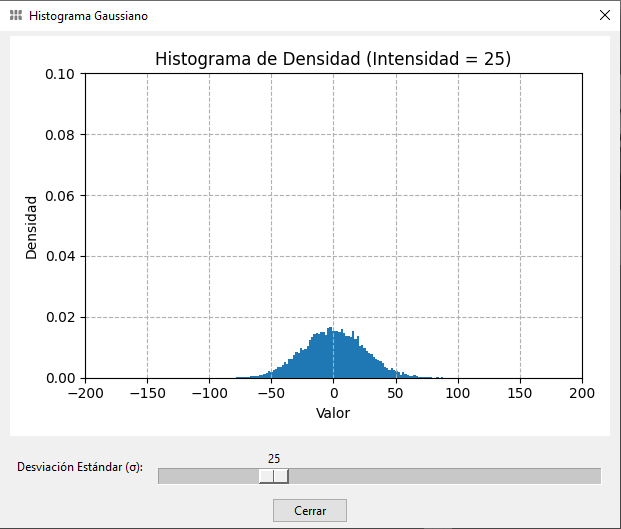
\includegraphics[width=\linewidth]{../results/dist_gauss}
		\captionof{figure}{Dist gaussiana}
	\end{minipage}\hfill
	% Segunda imagen
	\begin{minipage}{0.32\linewidth}
		\centering
		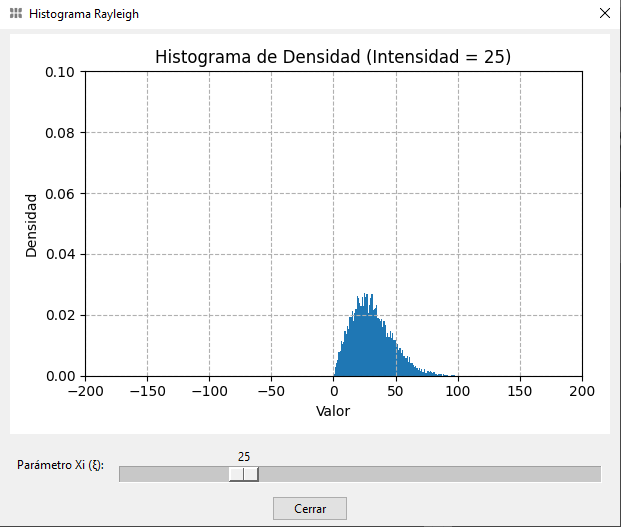
\includegraphics[width=\linewidth]{../results/dist_rayleigh}
		\captionof{figure}{Dist rayleigh}
	\end{minipage}\hfill
	% Tercera imagen
	\begin{minipage}{0.32\linewidth}
		\centering
		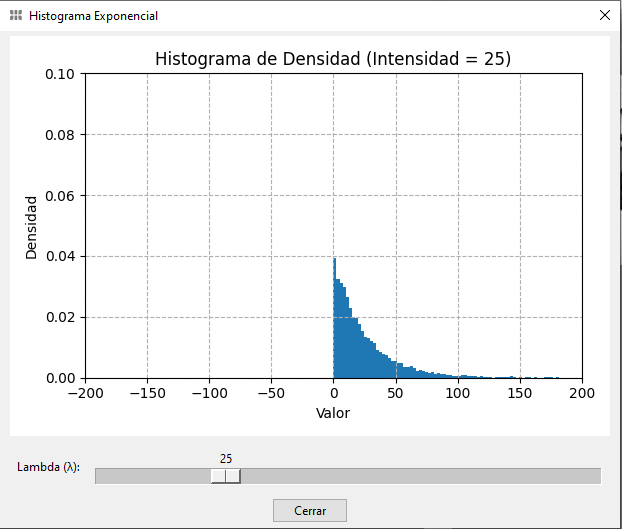
\includegraphics[width=\linewidth]{../results/dist_exponencial}
		\captionof{figure}{Dist exp}
	\end{minipage}
	
	\vfill
\footnotesize \textcolor{lightgray}{(*) Es conveniente probarlo en el programa para mayor interactividad.}
\end{frame}

\section{Ejercicio 8}

\begin{frame}
	\begin{center}
		\textcolor{unahurverde}{\textbf{Consigna 8:}}
	\end{center}
	\justifying
	
	Utilizando los generadores del punto anterior, implementar los siguientes puntos para agregar ruido a una imagen.
	
	\begin{enumerate}[label=\alph*)]
		\item Contaminar un porcentaje de una imagen con ruido Gaussiano aditivo.
		\item Contaminar un porcentaje de una imagen con ruido Rayleigh multiplicativo.
		\item Contaminar un porcentaje de una imagen con ruido exponencial multiplicativo.
	\end{enumerate}
	
	\vspace{0.3cm}
	
	El porcentaje de contaminación y los parámetros del generador deben ser parámetros de entrada.
\end{frame}

\begin{frame}[fragile]{Código}
	\justifying
	Para aplicar el ruido en la imagen utilizaremos la siguiente función:
	
	\begin{lstlisting}[language=Python]
def _aplicar_ruido(self, imagen, tipo, vector_ruido, d):
	imagen_np = np.array(imagen).astype(float)
	m, n, _ = imagen_np.shape
	
	# Cantidad de píxeles contaminados
	num_contaminados = int((d * (m * n)) / 100)
	# Indices (i, j) de los píxeles contaminados
	D = np.unravel_index(np.random.choice(m * n, num_contaminados, replace=False),(m, n))
	
	if tipo == "Aditivo": imagen_np[D] += vector_ruido
	elif tipo == "Multiplicativo": imagen_np[D] *= vector_ruido
	
	resultado_np = self._escalar_255(imagen_np)
	self.imagen_procesada = Image.fromarray(resultado_np)
	\end{lstlisting}
	
	\vfill
	\footnotesize \textcolor{lightgray}{(*) np.random.choice (ver \cite{numpy-random.choice}). np.unravel\_index (ver \cite{numpy-unravel-index}).}
\end{frame}

\section{Ejercicio 9}

\begin{frame}
	\begin{center}
		9) Implementar una función que devuelva el histograma de niveles de gris de una imagen.
	\end{center}
\end{frame}

\section{Ejercicio 10}

\begin{frame}
	\begin{center}
		10) Implementar una función que devuelva el histograma de niveles de gris de una imagen.
	\end{center}
\end{frame}

\section{Ejercicio 11}

\begin{frame}
	\begin{center}
		11) Implementar una función que devuelva el histograma de niveles de gris de una imagen.
	\end{center}
\end{frame}

\section{Ejercicio 12}

\begin{frame}
	\begin{center}
		12) Implementar una función que devuelva el histograma de niveles de gris de una imagen.
	\end{center}
\end{frame}

\section{Bibliografía}
	
	\begin{frame}{Referencias}
		\tiny
		\begin{thebibliography}{10}
			\beamertemplatebookbibitems
			\bibitem{numpy-broadcasting}
			NumPy Documentation: Broadcasting. 
			\newblock \url{https://numpy.org/doc/stable/user/basics.broadcasting.html}
			
			\bibitem{numpy-where}
			NumPy Documentation: numpy.where. 
			\newblock \url{https://numpy.org/doc/stable/reference/generated/numpy.where.html}
			
			\bibitem{numpy-bincount}
			NumPy Documentation: numpy.bincount. 
			\newblock \url{https://numpy.org/doc/stable/reference/generated/numpy.bincount.html}
			
			\bibitem{numpy-sum}
			NumPy Documentation: numpy.sum. 
			\newblock \url{https://numpy.org/doc/stable/reference/generated/numpy.sum.html}
			
			\bibitem{numpy-cumsum}
			NumPy Documentation: numpy.cumsum. 
			\newblock \url{https://numpy.org/doc/stable/reference/generated/numpy.cumsum.html}
			
			\bibitem{numpy-unravel-index}
			NumPy Documentation: numpy.unravel\_index. 
			\newblock \url{https://numpy.org/doc/stable/reference/generated/numpy.unravel_index.html}
			
			\bibitem{numpy-random.choice}
			NumPy Documentation: numpy.random.choice. 
			\newblock \url{https://numpy.org/doc/stable/reference/random/generated/numpy.random.choice.html}
		\end{thebibliography}
	\end{frame}
	
	\begin{frame}{}
		\centering
		{\huge ¡Gracias!}\\
		\vspace{1cm}
		
\includegraphics[width=0.2\textwidth]{UNAHUR.png}
	\end{frame}
	
\end{document}
